\chapter{Installer le logiciel}

\section{Consultez la documentation du framework !}

Le logiciel a été conçu à partir du framework \textit{Prototypephp}. La documentation associée \cite{pphp-doc} récapitule l'ensemble des informations nécessaires pour réaliser l'installation générale (configuration du serveur, définition des droits d'accès, etc.).

De nombreuses reprises figurent ici, mais il n'est pas inutile de se référer au document d'origine. Seuls les exemples dédiés au logiciel sont présentés, mais d'autres informations utiles pourront y être piochées.

\section{Configuration du serveur}
La configuration est donnée pour un serveur Linux fonctionnant avec Ubuntu 16.04 LTS Server. Elle peut bien sûr être adaptée à d'autres distributions Linux. Par contre, rien n'a été prévu pour faire fonctionner l'application directement dans une plate-forme windows, même si, en théorie, cela devrait être possible.

\subsection{Configuration d'Apache}
Les modules suivants doivent être activés :
\begin{lstlisting}
a2enmod ssl
a2enmod headers
a2enmod rewrite
\end{lstlisting}

\subsection{Modules PHP nécessaires}
Modules complémentaires nécessaires :
\begin{itemize}
\item \textit{php-mbstring}
\item \textit{php-pgsql}
\item \textit{php-xdebug} pour les phases de mise au point.
\end{itemize}
La génération des étiquettes nécessite les paquetages suivants :
\begin{itemize}
\item \textit{php-gd} (ou \textit{php5-gd} pour les serveurs en version 5)
\item \textit{fop} (qui inclut des bibliothèques java)
\end{itemize}

Le stockage et l'affichage des photos nécessite :
\begin{itemize}
\item \textit{php-imagick} (ou \textit{php5-imagick} pour les serveurs en version 5)
\end{itemize}

\subsection{Configuration de l'hôte virtuel et de SSL}
L'application ne fonctionne qu'en mode SSL, les cookies de session n'étant pas transmis sur des liens non chiffrés. Voici un exemple de configuration à insérer dans le fichier \textit{/etc/apache2/sites-available/default-ssl}
\begin{lstlisting}
    <Directory /var/www/html>
        Options FollowSymLinks MultiViews
        AllowOverride all
        Order allow,deny
        allow from all
    </Directory>

    SSLProtocol All -SSLv2 -SSLv3
    SSLHonorCipherOrder On
    SSLCipherSuite ECDHE-RSA-AES128-SHA256:AES128-GCM-SHA256:HIGH:!MD5:!aNULL:!EDH:!RC4
    SSLCompression off
\end{lstlisting}

La chaîne \textit{SSLCipherSuite} est donnée à titre d'exemple, d'autres configurations plus modernes peuvent être implémentées \cite{tls}.

Pour activer le mode SSL dans Apache :
\begin{lstlisting}
chmod -R g+r /etc/ssl/private
usermod www-data -a -G ssl-cert
a2ensite default-ssl
service apache2 restart
\end{lstlisting}


\subsection{Configuration du dossier d'installation}

\subsubsection{Mécanisme pour faire cohabiter plusieurs instances avec le même code}

Il est possible d'utiliser le même code applicatif pour alimenter des bases de données différentes (ou des données stockées dans des schémas différents). Cette fonctionnalité est basée sur l'attribution d'entrées DNS différentes. 

Le mécanisme est décrit dans le schéma \ref{dnsmultiple}, page \pageref{dnsmultiple}.

\begin{figure}[H]
\label{dnsmultiple}
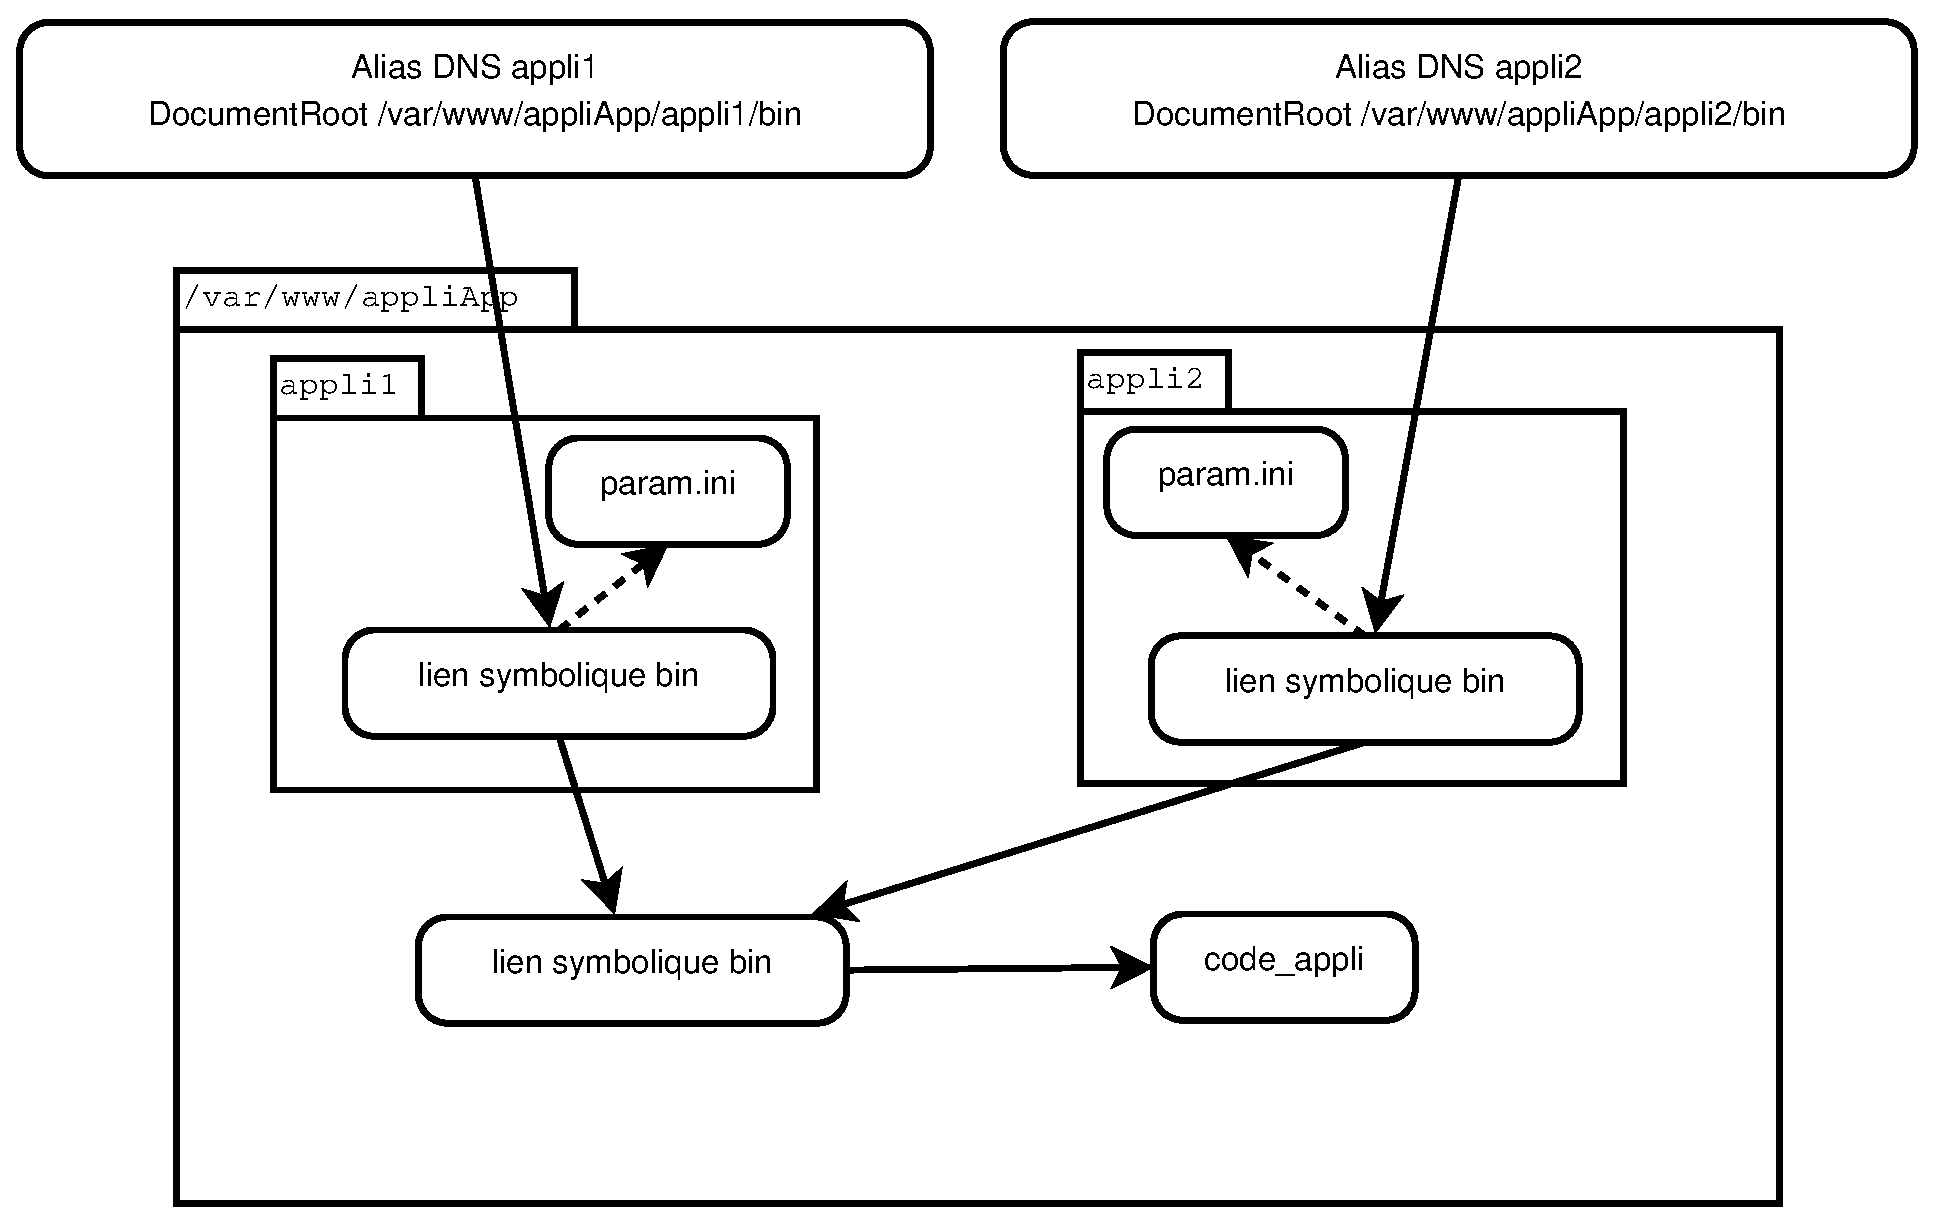
\includegraphics[width=\linewidth]{images/dnsmultiple}
\caption{Schéma général d’implémentation pour utiliser le même code avec des noms d’application et des jeux de données différents}
\end{figure}

Dans le paramétrage de l’alias DNS (en principe, dans \textit{/etc/apache2/sites-available}), l’application pointe vers le dossier \textit{/var/www/appliApp/appli1/bin}. \textit{/var/www} correspond à la racine du site web, \textit{appliApp} au dossier racine de l’application, \textit{appli1} au dossier spécifique de l’alias DNS. Ce dossier \textit{appli1} ne contient que deux fichiers : \textit{param.ini}, qui contient les paramètres spécifiques, et \textit{bin}, qui est un lien symbolique vers le dossier \textit{../bin}.

Le dossier \textit{../bin} (donc, dans\textit{ /var/www/appliApp}) est lui aussi un alias qui pointe vers le code réel de l’application, ici \textit{code\_appli}. Le fichier \textit{param.inc.php} décrit l’entrée suivante : 
\begin{lstlisting}
$paramIniFile = "../ param . ini "; 
\end{lstlisting}

Le fichier \textit{param.ini} sera cherché dans le dossier parent du code de l’application, c’est à dire soit dans \textit{appli1}, soit dans \textit{appli2} dans cet exemple. Il suffit qu’il contienne les paramètres adéquats pour rendre l’application utilisable dans des contextes différents à partir du même code initial.



Le fichier \textit{param.ini} est le dernier qui est traité par l'application pour récupérer les paramètres.Ceux-ci sont lus dans l'ordre suivant :

\textbf{param/param.default.inc.php $\rightarrow$ param/param.inc.php $\rightarrow$ ../param.ini}

\textit{param.ini} contiendra les entrées spécifiques liées au DNS utilisé pour accéder à l'application, en principe tout ou partie de celles-ci :
\begin{lstlisting}
APPLI_titre=Gestion des collections EABX
BDD_schema=col, public, gacl
BDD_login=compte_de_connexion
BDD_passwd=mot_de_passe_de_connexion
BDD_dsn=pgsql:host=serveur;dbname=base_de_donnees;sslmode=require
GACL_aco=col
APPLI_code=proto
\end{lstlisting}



\subsubsection{Droits à attribuer au serveur web}

\section{Configurer l'application}

L'application est configurable par l'intermédiaire de trois fichiers, comme nous venons de le voir :

\textbf{param/param.default.inc.php $\rightarrow$ param/param.inc.php $\rightarrow$ ../param.ini}

Le premier fichier contient les paramètres par défaut. Il est systématiquement fourni à chaque nouvelle version de l'application.

Le second est spécifique de l'implémentation. Il comprend notamment les informations liées à la connexion à la base de données, à la méthode d'identification, ou à la recherche des attributs dans l'annuaire LDAP. 

le troisième est destiné à traiter la possibilité d'accéder, à partir du même code applicatif, à plusieurs bases de données différentes (\textit{cf.} \ref{dnsmultiple} \textit{\nameref{dnsmultiple}}).

Voici les principaux paramètres utilisés :

\subsection{Connexion à la base de données}

Dans la pratique, deux connexions sont nécessaires : l'une pour accéder à la base des droits, l'autre aux données proprement dites. Voici les paramètres à définir :

\begin{longtable}{|p{5cm}|p{10cm}|}
\hline
\textbf{Variable} & \textbf{Signification} \\
\hline
\endhead
BDD\_login & compte de connexion à la base de données \\
\hline
BDD\_passwd & mot de passe associé\\
\hline
BDD\_dsn & adresse de la base de données sous forme normalisée\\
\hline
BDD\_schema & schéma utilisé (plusieurs schémas peuvent être décrits, en les séparant par une virgule - fonctionnement propre à Postgresql)\\
\hline
GACL\_dblogin & compte de connexion à la base de données des droits\\
\hline
GACL\_dbpasswd & mot de passe associé\\
\hline
GACL\_dsn & adresse normalisée \\
\hline
GACL\_schema & schéma utilisé\\
\hline
GACL\_aco & nom du code de l'application utilisé dans la gestion des droits\\
\hline
\caption{Variables utilisées pour paramétrer les connexions}
\end{longtable}

\subsection{Identification des utilisateurs}

\begin{longtable}{|p{5cm}|p{10cm}|}
\hline
\textbf{Variable} & \textbf{Signification} \\
\hline
\endhead
ident\_type & Type d'identification supporté. L'application peut gérer \textbf{BDD} (uniquement en base de données),\textbf{LDAP} (uniquement à partir d'un annuaire LDAP) \textbf{LDAP-BDD} (d'abord identification en annuaire LDAP, puis en base de données), et \textbf{CAS} (serveur d'identification \textit{Common Access Service})\\
\hline
CAS\_plugin & Nom du plugin utilisé pour une connexion CAS \\
\hline
CAS\_address & Adresse du serveur CAS\\
\hline
CAS\_port & Systématiquement 443 (connexion chiffrée)\\
\hline
LDAP & tableau contenant tous les paramètres nécessaires pour une identification LDAP \\
\hline
privateKey & clé privée utilisée pour générer les jetons d'identification \\
\hline
pubKey & clé publique utilisée pour générer les jetons d'identification \\
\hline
tokenIdentityValidity & durée de validité, en secondes, des jetons d'identification\\
\hline
\caption{Variables utilisées pour paramétrer l'identification}
\end{longtable}

\subsection{Configuration de l'accès à l'annuaire LDAP}

Les paramètres LDAP sont stockés dans un tableau :
\begin{lstlisting}
$LDAP = array(
		"address"=>"localhost",
		"port" => 389,
		"rdn" => "cn=manager,dc=example,dc=com",
		"basedn" => "ou=people,ou=example,o=societe,c=fr",
		"user_attrib" => "uid",
		"v3" => true,
		"tls" => false,
		"groupSupport"=>true,
		"groupAttrib"=>"supannentiteaffectation",
		"commonNameAttrib"=>"displayname",
		"mailAttrib"=>"mail",
		'attributgroupname' => "cn",
		'attributloginname' => "memberuid",
		'basedngroup' => 'ou=example,o=societe,c=fr'
);
\end{lstlisting}


L'application peut non seulement identifier les utilisateurs auprès de l'annuaire LDAP, mais également récupérer les groupes auxquels ils appartiennent dans celui-ci.

Voici les paramètres à indiquer dans ce cas de figure : 
\begin{longtable}{|p{5cm}|p{10cm}|}
\hline
\textbf{Variable} & \textbf{Signification} \\
\hline
\endhead
address &  adresse de l'annuaire\\
\hline
port & 389 en mode non chiffré, 636 en mode chiffré\\
\hline
rdn & compte de connexion, si nécessaire \\
\hline
basedn & base de recherche des utilisateurs\\
\hline
user\_attrib & nom du champ contenant le login à tester\\
\hline
v3 & toujours à \textit{true}\\
\hline
tls & \textit{true} en mode chiffré\\
\hline
groupSupport & \textbf{true} si l'application recherche les groupes d'appartenance du login dans l'annuaire\\
\hline
groupAttrib & Nom de l'attribut contenant la liste des groupes d'appartenance\\
\hline
commonNameAttrib & Nom de l'attribut contenant le nom de l'utilisateur\\
\hline
mailAttrib & Nom de l'attribut contenant l'adresse mail de l'utilisateur\\
\hline
attributgroupname & Attribut contenant le nom du groupe lors de la recherche des groupes (cn par défaut)\\
\hline
attributloginname & attribut contenant les membres d'un groupe\\
\hline
basedngroup & base de recherche des groupes \\
\hline
\caption{Variables utilisées pour paramétrer l'accès à l'annuaire LDAP}
\end{longtable}

\subsection{Paramètres spécifiques}

\begin{longtable}{|p{5cm}|p{10cm}|}
\hline
\textbf{Variable} & \textbf{Signification} \\
\hline
\endhead
GACL\_aco & nom du code de l'application utilisé dans la gestion des droits (\textit{cf.} \ref{droits} \textit{\nameref{droits}}, page \pageref{droits} )\\
\hline
APPLI\_code & Code interne de l'application. \textbf{Ce code est essentiel} : il sera inscrit dans les codes-barres générés, pour s'assurer qu'un échantillon est bien issu de la base de données concernée\\
\hline
\caption{Variables spécifiques}
\end{longtable}

\section{Créer la base de données}
